\chapter{Sicherheitsdienste}\label{Sicherheitsdienste}

In den vorherigen Kapiteln wurden Angriffsmöglichkeiten und die Anforderungen an ein verteiltes System untersucht. In diesem Kapitel erfolgt eine Konkretisierung der Sicherheitsdienste, die
ein verteiltes System bereitstellen muss um als sicher zu gelten. Dieses Kapitel erklärt die unterschiedlichen Dienste und stellt sie anschaulich anhand von Beispielen dar.

\section{Vertraulichkeit}
\section{Authentifizierung}

Authentifizierung sogrt dafür, dass ein Benutzer gegenüber einem System verifiziert werden kann.
Der Begriff der Authentifizierung wird oft synonym mit den Begriffen Authentisierung und Autorisierung verwendet. 
Die Authentifizierung lässt sich in weitere Bestandteile untergliedern. Der erste Bestandteil ist die Authentisierung, 
wobei der Benutzer gegenüber dem System eine Identität vorgibt, die von diesem bestätigt werden soll. 
Auf die Authentisierung folgt anschließend die Authentifizierung. Bei dem Authentifizierungsvorgang werden die vom Nutzer 
eingegebenen Daten, also seine angegebene Identität, überprüft. Ist die Überprüfung abgeschlossen folgt die 
Autorisierung. Die Autorisierung ist für die Zuteilung der Zugriffsrechte verantwortlich. 
Durch den Prozess der Authentifizierung wird eine Identität an ein Subjekt/ Entität gebunden. 
Das Binden der Identität berechtigt den Benutzer bestimmte Dienste in Anspruch nehmen zu können. 
\newline
Es gibt verschiedene Arten wie eine Authentifizierung durchgeführt werden kann:
\begin{figure}[H]
    \centering
    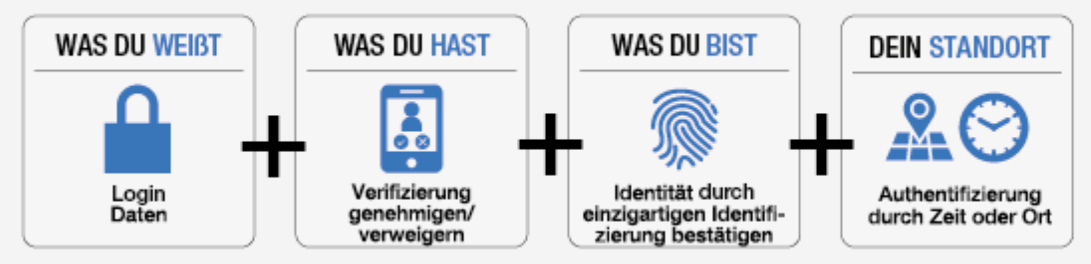
\includegraphics[width=\textwidth]{images/authent_pos1.png}
    \caption[Authentifizierungsarten]{Authentifizierungsarten} 
    \label{Authentifizierungsarten}
\end{figure} 

Im Zusammenhang mit verteilten Systemen im Internet ist die Authentifizierung durch Wissen,
also Benutzername und Passwort, weit verbreitet. 
Das Passwort besteht dabei meistens aus einer Zeichenkombination und wird über einen geschützten Kanal ausgetauscht. 
Besonders bei Diensten im Internet bietet sich die Verwendung von Hyper-Text-Transfer-Protocol-Secure (HTTPS), statt
des ungesicherten Hyper-Text-Transfer-Protocol (HTTP) an.
Das auslesen der Benutzerdaten aus dem Netzwerkverkehr ist so nicht mehr möglich. 
Mit Verwendung eines sicheren Protokolles für die Übermittlung der Daten ist die Übertragung zwischen den Systemen 
als Angriffsvektor ausgeschlossen. 
Sind die Daten erfolgreich und sicher an das Serversystem übermittelt worden müssen diese in bestimmter Form 
(bspw. in einer Datenbank) persistiert werden. 
Das festhalten der Daten im Klartext würde die Datenbank zu einem sehr lohnenden Ziel machen, da die Daten 
an einer stelle gesammelt einsehbar wären. 
Aus diesem Grund benutzt man verschiedene Verschlüsselungsfunktionen um zumindest die Passwörter in eine Form zu bringen,
die nicht wieder re-konstruiert werden kann. Das Anwenden der Verschlüsselungsfunktion wird 
als Hashing bezeichnet. Gehashte Passwörter in der Datenbank bieten eine notwendige Sicherheit um die Daten in sicherer Form 
dauerhaft zu abzulegen. Abgesehen von der Authentifizierung durch Wissen mittels Benutzername und Passwort gibt es die Möglichkeit sich durch 
Besitzt, Identität oder den Standort zu Authentifizieren. 
Besonders interessant für zusätzliche Sicherheit auf Client-Seite können die 
Authentifizierungsmöglichkeiten kombiniert werden. Die Kombination von bspw. einer Authentifizierung durch Wissen und von Besitz 
wird als 2-Faktor-Authentifizierung bezeichnet. Gelangt ein Angreifer an ein Passwort hat er so ohne die entpsrechende zweite 
Authentifizierungsmethode keine Möglichkeit die Identität des Benutzers anzunehmen. 

\section{Integrität}
\section{Nicht-Anfechtbarkeit}
\section{Zugriffssteuerung/Autorisierung}
\section{Verfügbarkeit}